\documentclass[xcolor={dvipsnames}]{beamer}
\usepackage[utf8]{inputenc}

\usetheme{Madrid}
\usecolortheme{default}
\setbeamertemplate{enumerate items}[default]
\setbeamercolor*{structure}{bg=white,fg=black}

%Hyphenation rules
%--------------------------------------
\usepackage{hyphenat}
%--------------------------------------
\usepackage[english, russian]{babel}
\documentclass{standalone}
\usepackage[pdf]{graphviz}

\usepackage{svg}
\usepackage{amsmath}


%%% Helper code for Overleaf's build system to
%%% automatically update output drawings when
%%% code in a \digraph{...} is modified
\usepackage{xpatch}
\makeatletter
\newcommand*{\addFileDependency}[1]{% argument=file name and extension
  \typeout{(#1)}
  \@addtofilelist{#1}
  \IfFileExists{#1}{}{\typeout{No file #1.}}
}
\makeatother
\xpretocmd{\digraph}{\addFileDependency{#2.dot}}{}{}


% \setbeamercolor*{palette primary}{use=structure,fg=white,bg=structure.fg}
% \setbeamercolor*{palette secondary}{use=structure,fg=white,bg=structure.fg!75}
% \setbeamercolor*{palette tertiary}{use=structure,fg=white,bg=structure.fg!50!black}
% \setbeamercolor*{palette quaternary}{fg=white,bg=black}

% \setbeamercolor{section in toc}{fg=black,bg=white}
% \setbeamercolor{alerted text}{use=structure,fg=structure.fg!50!black!80!black}
% \setbeamercolor{frametitle}{bg=black,fg=white}

% \setbeamercolor{titlelike}{parent=palette primary,fg=structure.fg!50!black}
% \setbeamercolor{frametitle}{bg=gray!10!white,fg=black}

% \setbeamercolor*{titlelike}{parent=palette primary}

% \setbeamercolor{block title example}{bg=black,fg=white}

% \usepackage{times,url}

% \setbeamertemplate{footline}[frame number]
% \setbeamertemplate{footline}[frame number]{}

\setbeamertemplate{footline}{}

\setbeamertemplate{footline}
% {
%   \leavevmode%
%   \hbox{%
%   \begin{beamercolorbox}[wd=.333333\paperwidth,ht=2.25ex,dp=1ex,center]{author in head/foot}%
%     \usebeamerfont{author in head/foot}\insertsection
%   \end{beamercolorbox}%
%   \begin{beamercolorbox}[wd=.333333\paperwidth,ht=2.25ex,dp=1ex,center]{title in head/foot}%
%     \usebeamerfont{title in head/foot}\insertsubsection
%   \end{beamercolorbox}%
%   \begin{beamercolorbox}[wd=.333333\paperwidth,ht=2.25ex,dp=1ex,right]{date in head/foot}%
%     \usebeamerfont{date in head/foot}\insertshortdate{}\hspace*{2em}
%     \insertframenumber{} / \inserttotalframenumber\hspace*{2ex} 
%   \end{beamercolorbox}}%
%   \vskip0pt%
% }

%------------------------------------------------------------
%This block of code defines the information to appear in the
%Title page
\title[About Beamer] %optional
{Model Checking}

\subtitle{Модель Крипке для кофемашины DeLonge}

\author[] % (optional)
{Shurygin Anton Alexeevich}


% 右下角使用logo的方式
% \logo{\includegraphics[height=1cm]{overleaf-logo}} 

%End of title page configuration block
%------------------------------------------------------------





\begin{document}

%The next statement creates the title page.
\frame{\titlepage}



\section{Введение}

%---------------------------------------------------------
%Changing visivility of the text
\begin{frame}
\frametitle{Введение}

Последние несколько недель я только и существую с помощь кофемашины DeLonge. Поэтому я решил описать ее устройство, используя модель Крипке, поскольку пользовался ей достаточно.

\begin{figure}[h!]
    \begin{center}
    \begin{minipage}[h!]{0.3\linewidth}
        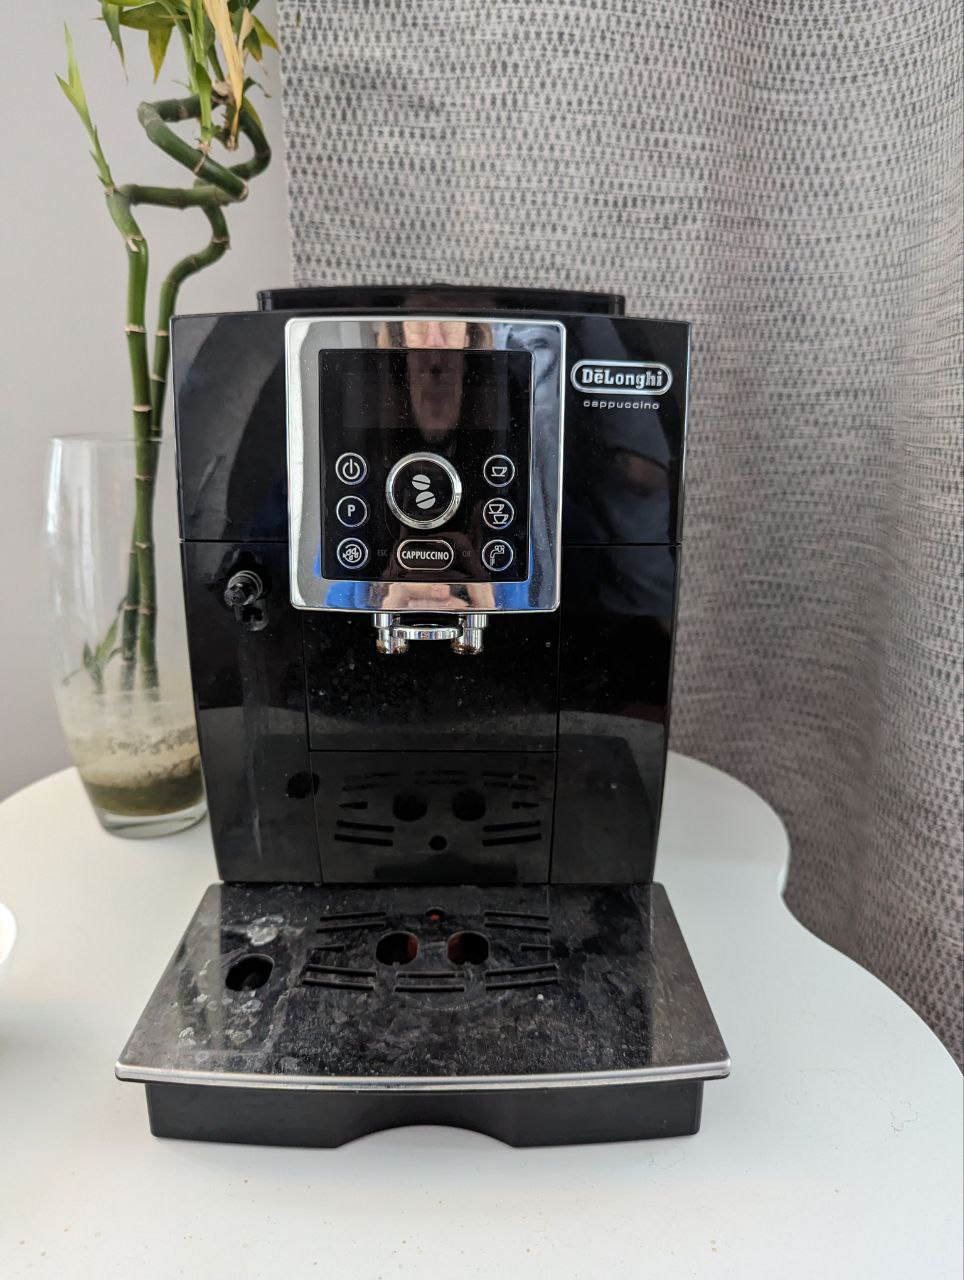
\includegraphics[width=1\linewidth]{pics/delonge1.jpg}
        \caption{Вид спереди} 
    \label{} 
    \end{minipage}
\hfill
    \begin{minipage}[h!]{0.4\linewidth}
        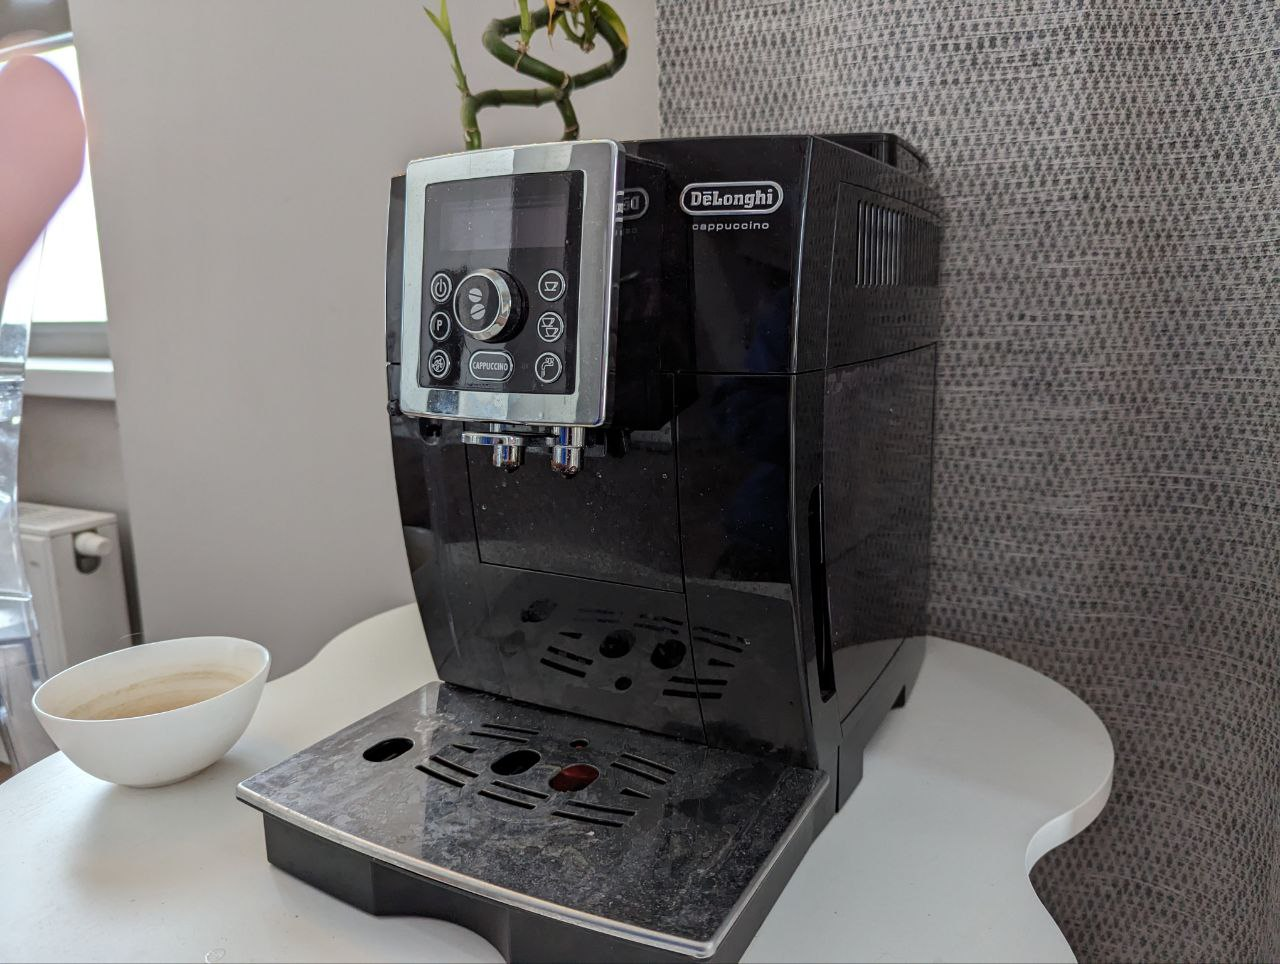
\includegraphics[width=1\linewidth]{pics/delonge2.jpg}
        \caption{Вид сбоку}
        \label{}
    \end{minipage}
    \end{center}
\end{figure}

\end{frame}

%---------------------------------------------------------


\begin{frame}
\frametitle{Введение}

Определим множество предикатов нашей системы $P = s, h, w, g, m$

\begin{itemize}
    \item $s$ - start, флаг запуска кофемашины, работу от сети
    \item $h$ - heated, флаг прогретости термопары кофемашины
    \item $w$ - water, флаг гарантирующий необходимого количества воды для работы
    \item $g$ - ground, флаг, гарантирующий свободное место в контейнере для гущи
    \item $g$ - ground, флаг, гарантирующий использования молока
\end{itemize}

\end{frame}


%---------------------------------------------------------
\begin{frame}
\frametitle{Введение}

Определим множество состояний нашей системы $S$

\begin{itemize}
    \item $S_0$ - кофемашина выключена
    \item $S_1$ - кофемашина подключена в сеть
    \item $S_2$ - кофемашина проверяет нынышнее значение воды
    \item $S_3$ - кофемашина проверяет заполненность контейнера для гущи 
    \item $S_4$ - кофемашина в режиме ожидания
    \item $S_5$ - приготовить кофе с молоком
    \item $S_6$ - приготовить черный кофе
    \item $S_7$ - кофемашина запрашивает очистить бак с молоком 
    \item $S_8$ - невалидное состояние, термпопара прогрелась до проверки количества воды
\end{itemize}

\end{frame}

%---------------------------------------------------------

\section{Second section}

%---------------------------------------------------------
%Highlighting text
\begin{frame}
\frametitle{Алгоритм функицонирования DeLonge}

\begin{figure}[h!]
            \begin{center}
			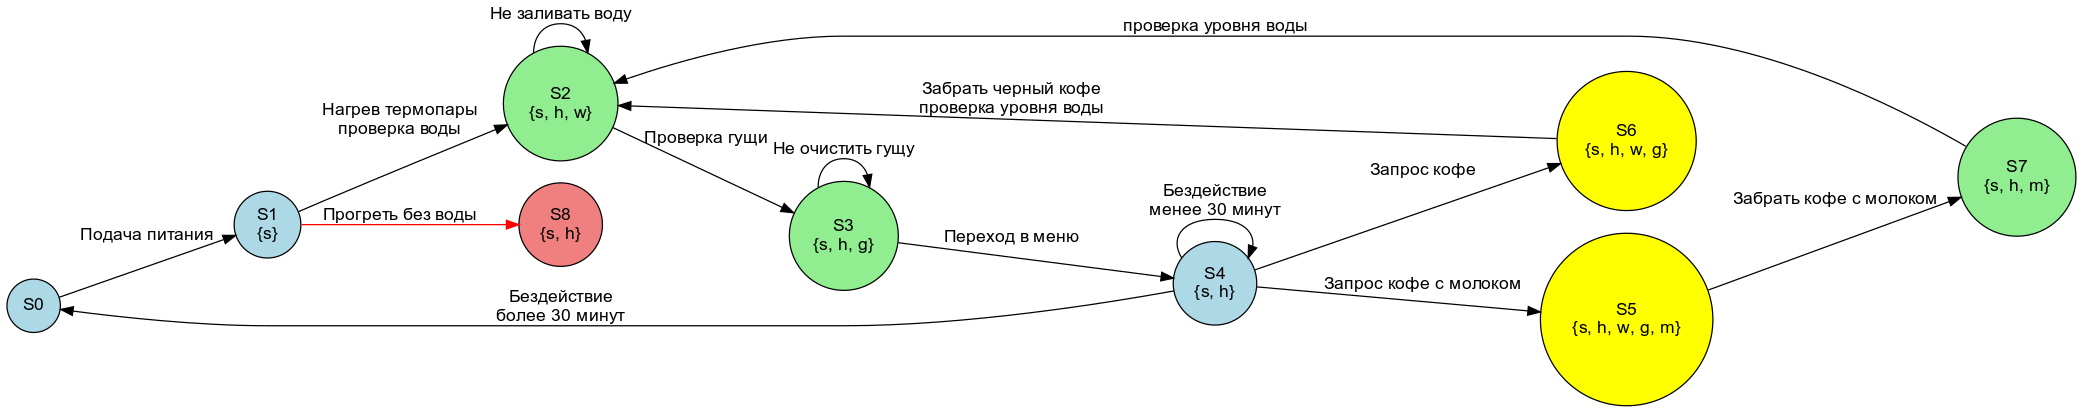
\includegraphics[width=1.0\linewidth]{pics/coffee.png}
			\caption{Граф переходов между состояниями}
			\end{center}
                \label{graph}
\end{figure}


\end{frame}
%---------------------------------------------------------


\begin{frame}
\frametitle{Cвойства safety}

    Свойства safety  с использованием темпоральной логики LTL:
\begin{enumerate}

\item Требование безопасности: После включения (s) и нагрева термопары (h), должна произойти проверка воды (w).
   LTL: $G((s \land h) \rightarrow Fw)$

\item Проверка гущи (g) должна произойти только после проверки воды (w):
   LTL: $G((w \rightarrow Fg))$

\item Проверка гущи (g) должна произойти только после включения (s) и нагрева термопары (h):
   LTL: $G((s \land h) \rightarrow Fg)$

\item Если контейнер с гущей (g) пуст, то после запроса кофе (в состоянии s, h, g) должен произойти переход в меню в режим ожидания (в состояние s, h):
   LTL: $G(((s \land h \land w \land g \land m) \rightarrow F(s \land h \land w \land m)))$

\item Если кофемашина выключена (s), то не должно произойти запроса кофе с молоком:
   LTL: $G(s \rightarrow \neg F(s \land h \land w \land g \land m))$

\end{enumerate}

    \end{frame}


\begin{frame}
\frametitle{Cвойства liveness}

Свойства liveness (живучести) в терминах темпоральной логики LTL:

\begin{enumerate}
    \item После нагрева термопары, должна произойти проверка гущи:
   LTL: $G(h \rightarrow Fg)$

    \item  После запроса  кофе кофе с молоком должна произойти очистка трубки с молоком:
   LTL: $G(((s \land h \land w \land g \land m) \rightarrow F(s \land h \land m))$


\end{enumerate}
    
    
\end{frame}


\begin{frame}
\frametitle{Нарушение свойства safety}

На рис.\ref{graph} указан красным цветом пример состояния, нарушающий одно свойство safety. Формализуем это как
$G(h \rightarrow \neg w)$ означает буквально "всегда верно, что если термопара нагрета, то вода не проверяется". Это невалидное состояние, так как нагрев термопары в начале должен быть предшествовать проверке воды для корректной работы кофейной машины.


\end{frame}
%---------------------------------------------------------


\end{document}